% !TeX document-id = {f19fb972-db1f-447e-9d78-531139c30778}
% !BIB program = biber
%\documentclass[handout]{beamer}
\documentclass[compress]{beamer}
\usepackage[T1]{fontenc}
\usepackage{pifont}
\usetheme[block=fill,subsectionpage=progressbar,sectionpage=progressbar]{metropolis} 

\usepackage{wasysym}
\usepackage{etoolbox}
\usepackage[utf8]{inputenc}

\usepackage{threeparttable}
\usepackage{subcaption}

\usepackage{tikz-qtree}
\setbeamercovered{still covered={\opaqueness<1->{5}},again covered={\opaqueness<1->{100}}}


\usepackage{listings}

\lstset{
	basicstyle=\scriptsize\ttfamily,
	columns=flexible,
	breaklines=true,
	numbers=left,
	%stepsize=1,
	numberstyle=\tiny,
	backgroundcolor=\color[rgb]{0.85,0.90,1}
}



\lstnewenvironment{lstlistingoutput}{\lstset{basicstyle=\footnotesize\ttfamily,
		columns=flexible,
		breaklines=true,
		numbers=left,
		%stepsize=1,
		numberstyle=\tiny,
		backgroundcolor=\color[rgb]{.7,.7,.7}}}{}


\lstnewenvironment{lstlistingoutputtiny}{\lstset{basicstyle=\tiny\ttfamily,
		columns=flexible,
		breaklines=true,
		numbers=left,
		%stepsize=1,
		numberstyle=\tiny,
		backgroundcolor=\color[rgb]{.7,.7,.7}}}{}


\usepackage[american]{babel}
\usepackage{csquotes}
\usepackage[style=apa, backend = biber]{biblatex}
\DeclareLanguageMapping{american}{american-UoN}
\addbibresource{../../literature.bib}
\renewcommand*{\bibfont}{\tiny}

\usepackage{tikz}
\usetikzlibrary{shapes,arrows,matrix}
\usepackage{multicol}

\usepackage{subcaption}

\usepackage{booktabs}
\usepackage{graphicx}

\graphicspath{{../../pictures/}}

\makeatletter
\setbeamertemplate{headline}{%
	\begin{beamercolorbox}[colsep=1.5pt]{upper separation line head}
	\end{beamercolorbox}
	\begin{beamercolorbox}{section in head/foot}
		\vskip2pt\insertnavigation{\paperwidth}\vskip2pt
	\end{beamercolorbox}%
	\begin{beamercolorbox}[colsep=1.5pt]{lower separation line head}
	\end{beamercolorbox}
}
\makeatother

\setbeamercolor{section in head/foot}{fg=normal text.bg, bg=structure.fg}



\newcommand{\question}[1]{
	\begin{frame}[plain]
	\begin{columns}
		\column{.3\textwidth}
		\makebox[\columnwidth]{
			
\includegraphics[width=\columnwidth,height=\paperheight,keepaspectratio]{../pictures/mannetje.png}}
		\column{.7\textwidth}
		\large
		\textcolor{orange}{\textbf{\emph{#1}}}
	\end{columns}
\end{frame}}

\newcommand{\instruction}[1]{\emph{\textcolor{gray}{[#1]}}}


\title[Big Data and Automated Content Analysis]{\textbf{A Practical Introduction to Machine Learning in Python} \\Day 1 - Monday  Morning\\ »Introduction«}
\author[Rupert Kiddle, Marieke van Hoof]{Rupert Kiddle \\ Marieke van Hoof \\ ~ \\ \footnotesize{r.t.kiddle@vu.nl   \\m.vanhoof@uva.nl} \\}
\date{September 16, 2024}
\institute[Gesis]{Gesis}

\begin{document}


\tikzstyle{block} = [rectangle, draw, fill=blue!20, 
text width=5em, text centered, rounded corners, minimum height=4em]
\tikzstyle{line} = [draw]
\tikzstyle{pijltje} = [draw, -latex']
\tikzstyle{cloud} = [draw, ellipse,fill=red!20, node distance=3cm,
minimum height=2em, text width=4em, text centered,]




\begin{frame}{}
\titlepage
\end{frame}

\begin{frame}{Today}
\tableofcontents
\end{frame}


\begin{frame} 
All course materials can be found at\ldots \\
~~~~~~~~\url{https://github.com/annekroon/gesis-machine-learning/fall-2024}
\end{frame}

\section{Introducing\ldots}
\subsection{\ldots the people}

\begin{frame} 
Introducing\ldots \\
~~~~~~~~\ldots the people
\end{frame}


\begin{frame}{Introducing\ldots} {\huge{Rupert}} \small{} 

\begin{columns}
	\column{.3\textwidth}
	\makebox[\columnwidth]{
		
\includegraphics[width=\columnwidth,height=\paperheight,keepaspectratio]{../pictures/rupert.jpg}}
	\column{.7\textwidth}
	Rupert Kiddle\\
	PhD Candidate: Computational Communication Science (RM SocSci, BSc PolSci, BSc Neurosci)\\
	\begin{itemize}
		%\item Studied Communication Science in M\"unster and at the VU 2003--2009
		%\item PhD candidate @ ASCoR 2009--2012
		\item Vrije University Amsterdam, Journalism
  \item interested in (digital) journalism, language modelling and news recommendation.
	\end{itemize}
	@rptkiddle \textbar r.t.kiddle@vu.nl 
\end{columns}
\end{frame}

\begin{frame}{Introducing\ldots} {\huge{Marieke}} \small{} 
\begin{columns}[] \column{.3\textwidth} \makebox[\columnwidth]{ 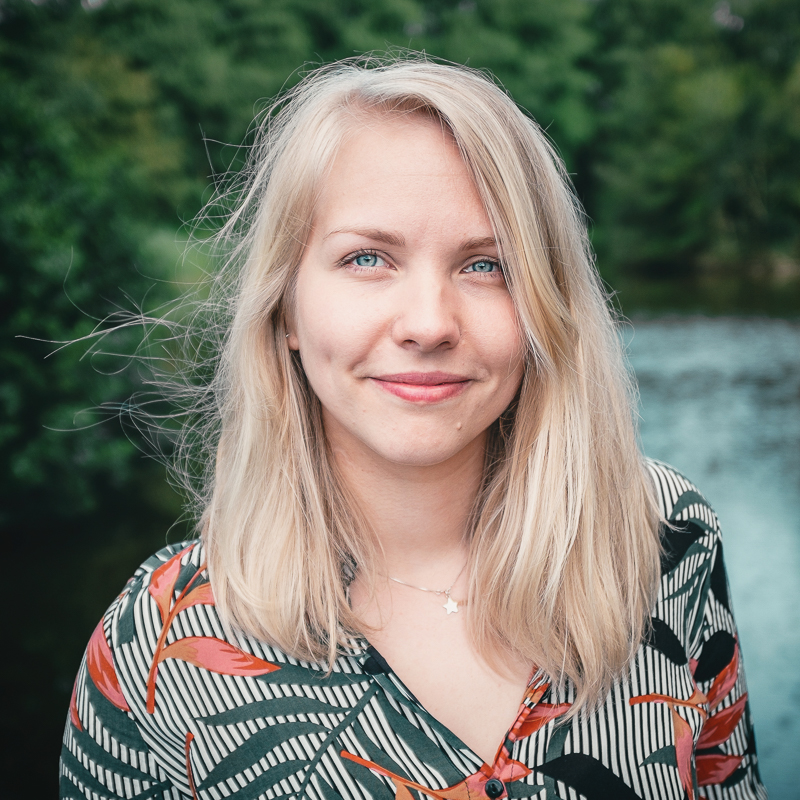
\includegraphics[width=\columnwidth,height=\paperheight,keepaspectratio]{../pictures/Marieke_klein.jpg}} \column{.7\textwidth} Marieke van Hoof \\ 
Postdoctoral researcher AI \& Politics (PhD PolCom, RM SocSci, BSc Sociology)
\begin{itemize} 
    \item Amsterdam School of Communication Research, University of Amsterdam
	\item Research focused on the role of AI and algorithms in political information diets
	\item Traditional methods (e.g., surveys, experiments) \& text analysis using automated approaches
\end{itemize} @marieke\_vh \textbar m.vanhoof@uva.nl 
\end{columns} 
\end{frame}

\begin{frame}{Introducing\ldots} {\huge{Damian \& Anne}} \small{} 
\begin{columns}[] \column{.5\textwidth} \makebox[\columnwidth]{ 
\includegraphics[width=\columnwidth,height=\paperheight,keepaspectratio]{../pictures/damian.jpg}} \\ prof. dr. Damian Trilling \\ Vrije Universiteit Amsterdam
\column{.5\textwidth} \makebox[\columnwidth]{ 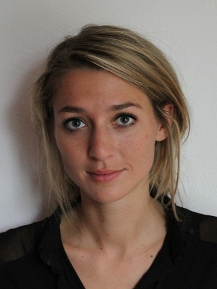
\includegraphics[width=\columnwidth,height=\paperheight,keepaspectratio]{../pictures/anne.jpg}} \\ dr. Anne Kroon \\ University of Amsterdam
\end{columns}
\end{frame}

\begin{frame}{Introducing\ldots}
{\huge{You}}
\small{}
\begin{columns}
\column{.3\textwidth}
\makebox[\columnwidth]{

\includegraphics[width=\columnwidth,height=\paperheight,keepaspectratio]{../pictures/mannetje.png}}
\column{.7\textwidth}
Your name?\\
Your background?\\
Your reason to follow this course?\\
Do you have a dataset you are working on?
\end{columns}
\end{frame}

\begin{frame}{Short poll}

Do you need
\begin{enumerate}[a]
	\item an intro
	\item a brief refresher
	\item nothing
\end{enumerate}

on

\begin{enumerate}[i]
	\item datatypes (int, float, string, lists, dictionaries)
	\item control flow statements (for, if, try/except)
	\item ways to run your code (notebooks vs IDE's vs text editors)
\end{enumerate}
?

\emph{We will try do adapt today's programme to your needs!}

\end{frame}

\section{Python: A language, not a program}


\begin{frame}[plain]
\makebox[\columnwidth]{
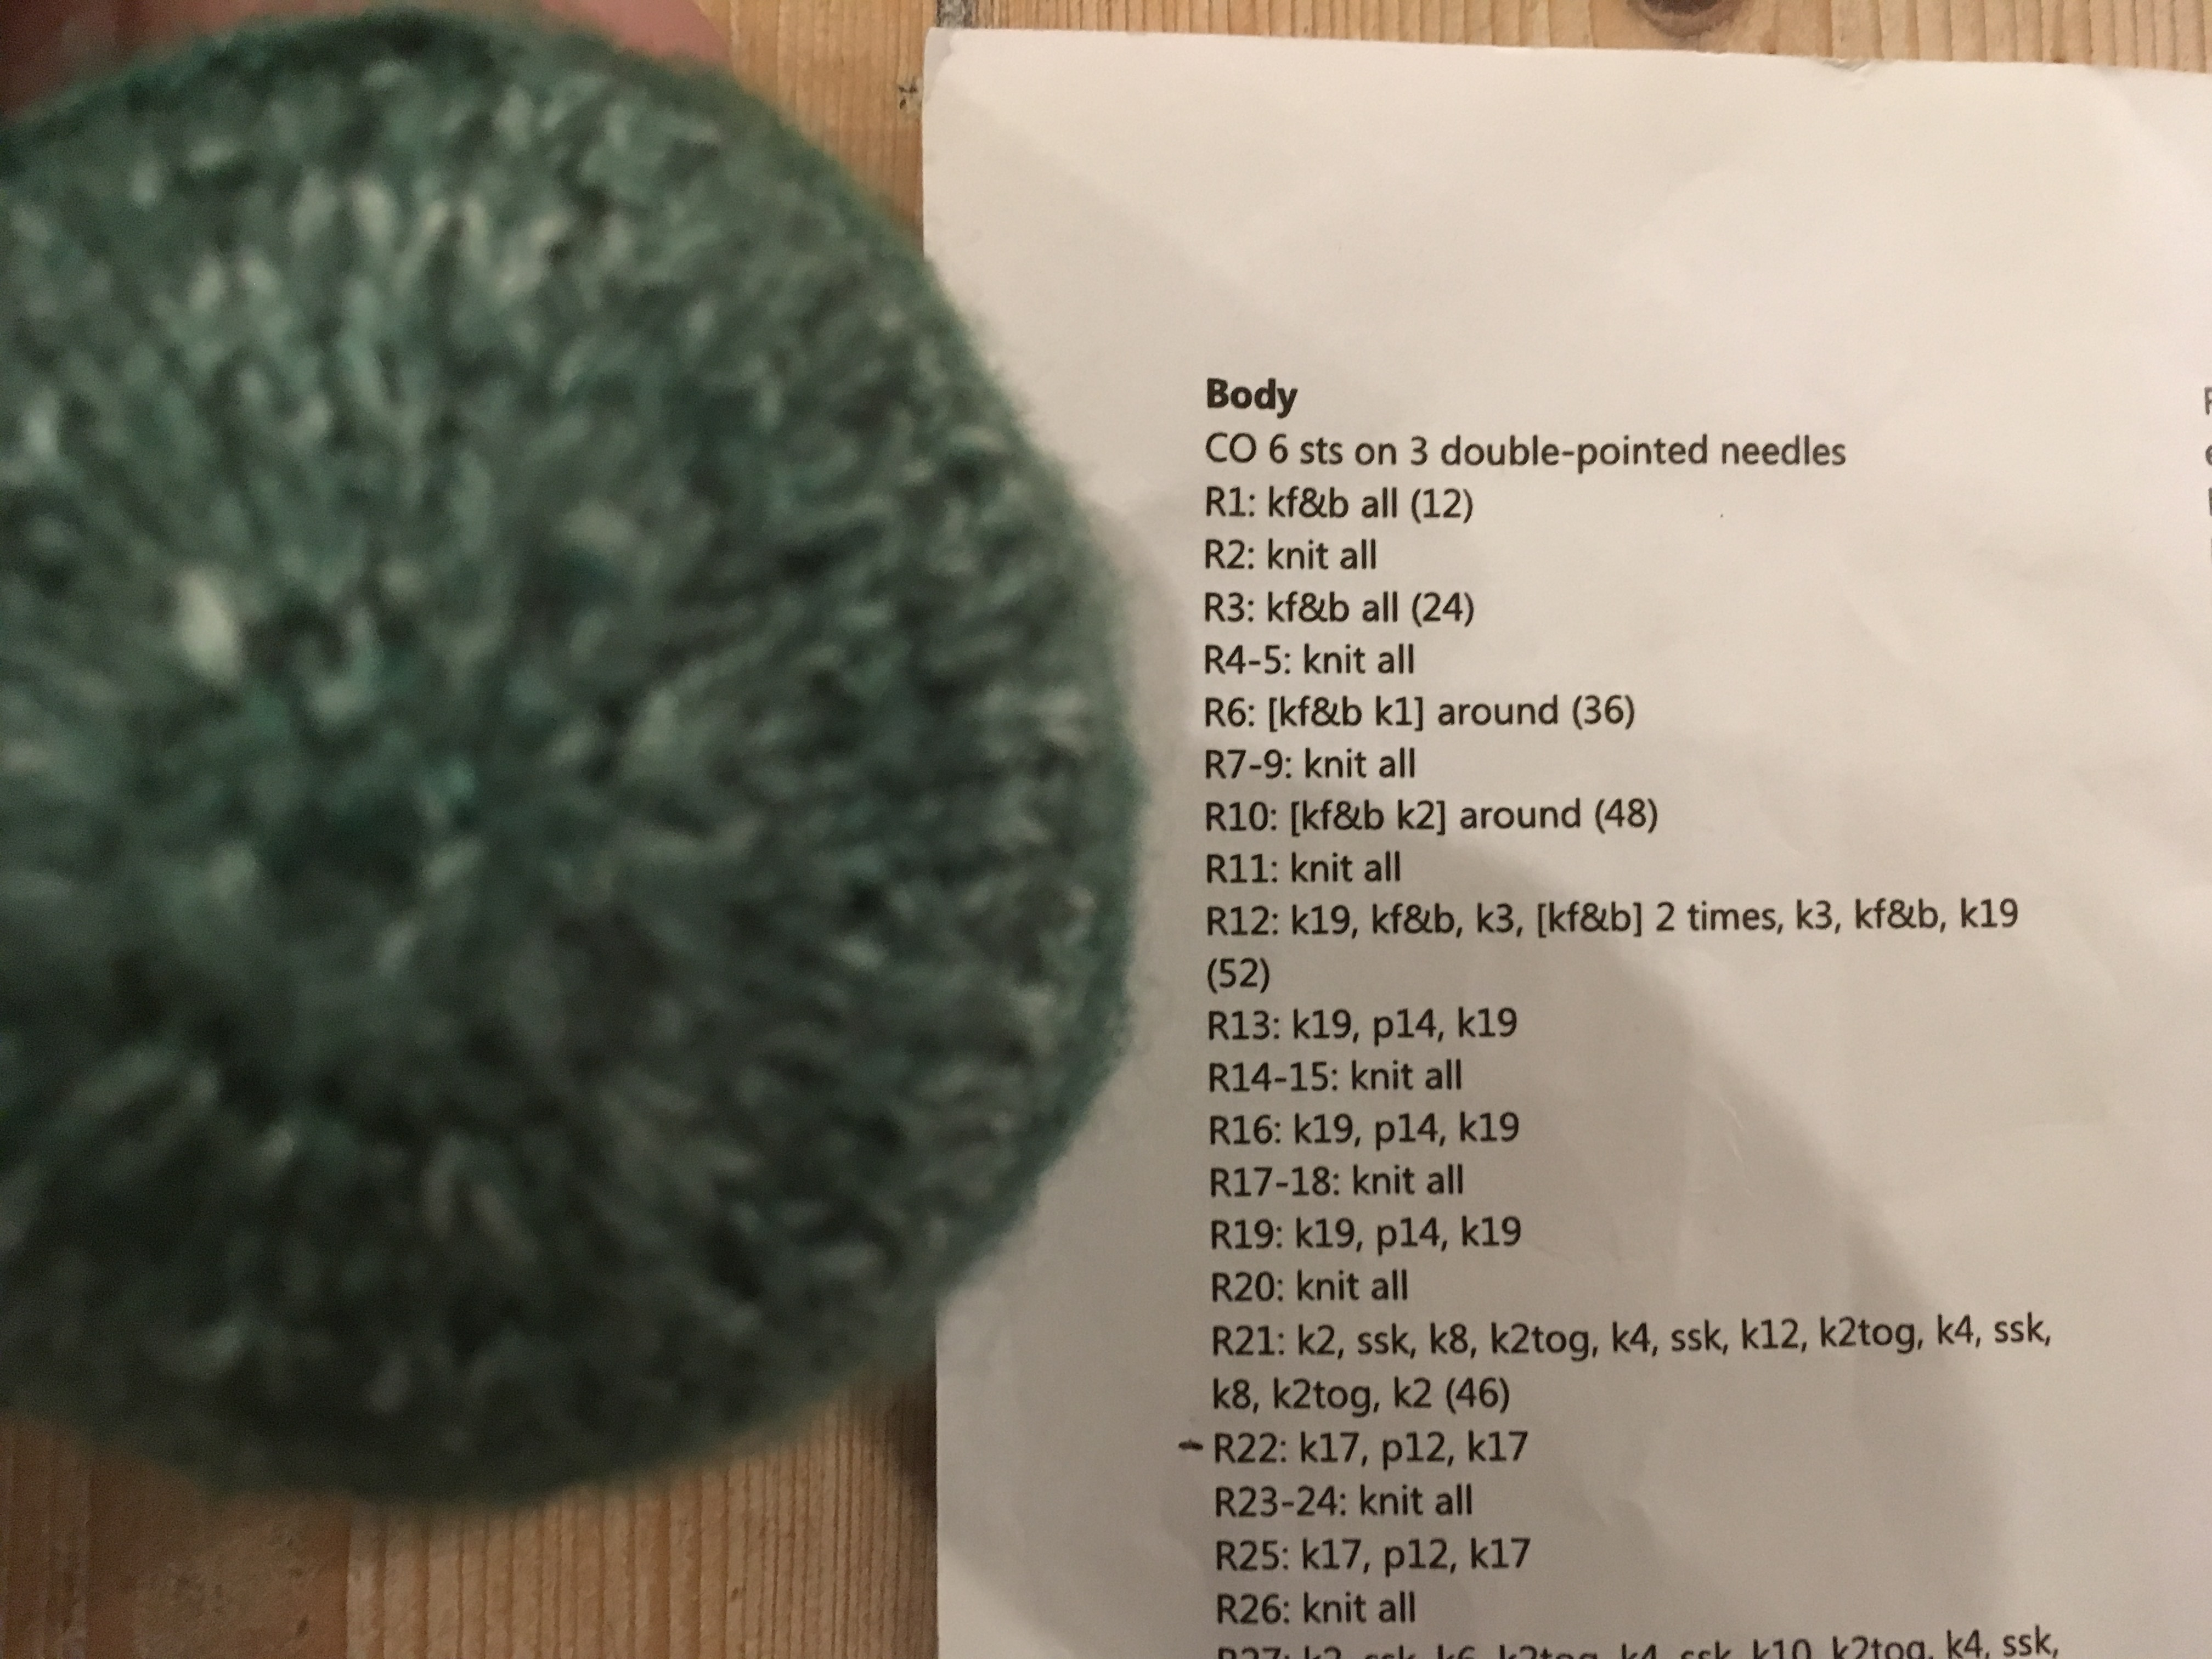
\includegraphics[width=\columnwidth,height=\paperheight,keepaspectratio]{../pictures/knitting.jpg}}
\footnotesize{An algorithm in a language that's a bit harder (I think) than Python}
\end{frame}



\begin{frame}{Python}
\begin{block}{What?}<1->
\begin{itemize}
\item A language, not a specific program
\item Huge advantage: flexibility, portability
\item One of \emph{the} languages for data analysis. \tiny{(The other one is R.)}
\onslide<2>{ \\\tiny{But Python is more flexible---the original version of Dropbox was written in Python. Some people say: R for numbers, Python for text and messy stuff.}}
\end{itemize}
\end{block}

\begin{block}{Which version?}<3->
We will use 3.10. Generally a good idea to use a recent version, but not the very latest. 
\end{block}
\end{frame}






\begin{frame}[plain]
\begin{tikzpicture}[node distance = 3cm, auto]
\node [cloud] (retrieve) {retrieve};
\node [cloud, right of=retrieve] (process) {process and/or enrich};
\node [cloud, right of=process] (analyze) {analyze\\ explain\\ predict};
\node [cloud, right of=analyze] (visualize) {communi-cate};


\path [pijltje] (retrieve)--(process);
\path [pijltje] (process)--(analyze);
\path [pijltje] (analyze)--(visualize);


\node [block, below of = retrieve] (retrievetech) {files\\ APIs\\ scraping};
\node [block, below of= process] (processtech) {NLP\\ sentiment\\ LDA\\ SML};
\node [block, below of=analyze] (analyzetech) {group comparisons; statistical tests and models};
\node [block, below of=visualize] (visualizetech) {visualizations and summary tables};


\path [pijltje] (retrievetech)--(processtech);
\path [pijltje] (processtech)--(analyzetech);
\path [pijltje] (analyzetech)--(visualizetech);


\node [block, below of = retrievetech, fill=green!20] (retrievepython) {glob\\ json \& csv\\ requests\\ lxml\\ \ldots};

\node [block, below of = processtech, fill=green!20] (processpython) {nltk\\ pattern \\ vader \\ gensim\\ scikit-learn \ldots};

\node [block, below of = analyzetech, fill=green!20] (analyzepython) {numpy/scipy\\ pandas\\ statsmodels\\ \ldots};

\node [block, below of = visualizetech, fill=green!20] (visualizepython) {pandas\\ matplotlib\\ seaborn\\ pyldavis\\ \ldots};

\path [line, dashed] (retrieve)--(retrievetech);
\path [line, dashed] (process)--(processtech);
\path [line, dashed] (analyze)--(analyzetech);
\path [line, dashed] (visualize)--(visualizetech);

\path [line, dashed] (retrievetech)--(retrievepython);
\path [line, dashed] (processtech)--(processpython);
\path [line, dashed] (analyzetech)--(analyzepython);
\path [line, dashed] (visualizetech)--(visualizepython);
\end{tikzpicture}
\end{frame}

\subsection{A good workflow}
\begin{frame}
	A good workflow
\end{frame}


\begin{frame}{Maximize transparency}
\begin{block}{Maximizing transparency of code and data}
	\begin{itemize}[<+->]
		\item Use openly accessible repository (e.g., Github)
		\item Store and preserve (pseudonymised) data at a secure environment (e.g., OSF)
		\item Create reusable workflows 
	\end{itemize}
\end{block}
\pause
\begin{exampleblock}{Advantages}
	\begin{itemize}[<+->]
		\item Reusable data and code
		\item Efficiency and credibility 
		\item Recognition of tools and data
	\end{itemize}
\end{exampleblock}

\end{frame}	

\subsection{Clean, high-quality code}
\begin{frame}{Develop components separately}
	\begin{block}{One script for downloading the data, one script for analyzing}
		\begin{itemize}[<+->]
			\item Avoids waste of resources (e.g., unnecessary downloading multiple times)
			\item Makes it easier to re-use your code or apply it to other data
		\end{itemize}
	\end{block}
\pause
\begin{block}{Start small, then scale up}
	\begin{itemize}[<+->]
		\item Take your plan and solve \textit{one} problem at a time (e.g., parsing a review page; or getting the URLs of all review pages)
		\item (for instance, by using functions [next slides])
	\end{itemize}
\end{block}

\end{frame}	

\begin{frame}{Develop components separately}
	\begin{block}{If you copy-paste code, you are doing something wrong}
		\begin{itemize}[<+->]
			\item Write loops!
			\item If something takes more than a couple of lines, write a function!
		\end{itemize}
	\end{block}
\end{frame}

\begin{frame}[plain, fragile]
Copy-paste approach\\ (ugly, error-prone, hard to scale up)
\begin{lstlisting}
allreviews = []

response = requests.get(`http://xxxxx')
tree =  fromstring(response.text)
reviewelements = tree.xpath(`//div[@class="review"]')
reviews = [e.text for e in reviewelements]
allreviews.extend(reviews)

response = requests.get(`http://yyyyy')
tree =  fromstring(response.text)
reviewelements = tree.xpath(`//div[@class="review"]')
reviews = [e.text for e in reviewelements]
allreviews.extend(reviews)
\end{lstlisting}
\end{frame}


\begin{frame}[plain, fragile]
Better: for-loop\\ (easier to read, less error-prone, easier to scale up (e.g., more URLs, read URLs from a file or existing list)
\begin{lstlisting}
allreviews = []

urls = [`http://xxxxx', `http://yyyyy']

for url in urls:
    response = requests.get(url)
    tree =  fromstring(response.text)
    reviewelements = tree.xpath(`//div[@class="review"]')
    reviews = [e.text for e in reviewelements]
    allreviews.extend(reviews)
\end{lstlisting}
\end{frame}


\begin{frame}[plain, fragile]
Even better: for-loop with functions\\ (main loop is easier to read, function can be re-used in multiple contexts)
\begin{lstlisting}
def getreviews(url):
    response = requests.get(url)
    tree =  fromstring(response.text)
    reviewelements = tree.xpath(`//div[@class="review"]')
    return [e.text for e in reviewelements]


urls = [`http://xxxxx', `http://yyyyy']

allreviews = []

for url in urls:
    allreviews.extend(getreviews(url))
\end{lstlisting}
\end{frame}

\subsection{Exercise}
\begin{frame}{Exercises}
\begin{block}{Did you pass?}
	\begin{itemize}
		\item Think of a way to determine for a list of  grades whether they are a pass (>5.5) or fail.
		\item Can you make that program robust enough to handle invalid input (e.g., a grade as 'ewghjieh')?
		\item How does your program deal with impossible grades (e.g., 12 or -3)?
		\item \ldots
	\end{itemize}
\end{block}
\end{frame}

\subsection{datatypes}
\begin{frame}{Datatypes}
\begin{block}{Low-level: Native python datatypes}
	\begin{itemize}[<+->]
		\item Booleans, integers, floats, strings, bytes, byte arrays
		\item Lists, typles, sets, dictionaries
	\end{itemize}
\end{block}
\pause
\begin{exampleblock}{Advantages }
	\begin{itemize}[<+->]
		\item fast, flexible
		\item allows for nested, unstructured data 
	\end{itemize}
\end{exampleblock}
\pause
\begin{alertblock}{Disadvantages }
	\begin{itemize}[<+->]
		\item can be more cumbersome: e.g., inserting a column
		\item less consistency checks
	\end{itemize}
\end{alertblock}
\end{frame}


\begin{frame}{Datatypes}
\begin{block}{Higher-level: importing modules}
	\begin{itemize}[<+->]
		\item e.g., numpy, pandas, seaborn 
	\end{itemize}
\end{block}
\pause
\begin{exampleblock}{Advantages}
	\begin{itemize}[<+->]
		\item useful convenience functionality, works very intuitively (for tabular data)
		\item easy, allows for pretty visualization
	\end{itemize}
\end{exampleblock}
\pause
\begin{alertblock}{Disadvantages }
	\begin{itemize}[<+->]
		\item not suited for one-dimensional or messy / deeply nested data
		\item when your data is very large (machine learning!!)
	\end{itemize}
\end{alertblock}
\end{frame}

\begin{frame}{Datatypes in this course}
In this week, we will mainly work with lower-level datatypes (as opposed to, for instance, pandas dataframes)
\begin{itemize}[<+->]
	\item Often, ML algorithms require native data types as input (i.e., lists, genertors)
	\item We have to seriously consider memory:
	\item Maybe size does not apply to your project yet, but in the future you might want to scale up. 
\end{itemize}	
\end{frame}

\subsection{Generators}
\begin{frame}{Generators}
\begin{block}{Generators}
	\begin{itemize}[<+->]
		\item We will work with \textit{generators} to deal with memory issues
		\item Generators behave like iterators: loops through elements of an object. 
	\end{itemize}
\end{block}
\pause
\begin{exampleblock}{Behavior of a generator}
	\begin{itemize}[<+->]
		\item Does not hold results in memory
		\item Only computes results at the moment you need them (i.e. lazy')
		\item You can only loop over your object ONCE.
	\end{itemize}
\end{exampleblock}
\end{frame}

\begin{frame}[plain, fragile]
Creating generators: Example 1 
\begin{lstlisting}
def my_generator(my_list):	
    for i in my_list:
        yield i
example_list = [1, 2, 3, 4]
gen1 = my_generator(example_list)        
next(gen1)
\end{lstlisting}
This will return:
\begin{lstlisting}
1
\end{lstlisting}
\end{frame}


\begin{frame}[plain, fragile]
Creating generators: Example 2 (shorter)
\begin{lstlisting}
my_list = [1,2,3,4]
gen = (i for i in my_list)
\end{lstlisting}
\end{frame}


\subsection{Scaling up}
\begin{frame}{Scaling up}
When considering datatypes, consider re-usability, scalability
	\begin{itemize}
		\item Use functions and classes to make code more readable and re-usable
		\item Avoid re-calculating values
		\item Think about how to minimize memory usage (e.g., Generators)
		\item Do not hard-code values, file names, etc., but take them as arguments
	\end{itemize}	
\end{frame}


\begin{frame}{Make it robust}
You cannot foresee every possible problem.\\
Most important: Make sure your program does not fail and loose all data just because something goes wrong at case 997/1000.
	\begin{itemize}
		\item Use \texttt{try/except} to explicitly tell the program how to handle errors
		\item Write data to files (or database) in between
		\item Use \texttt{assert len(x) == len(y}) for sanity checks
	\end{itemize}	
\end{frame}

\subsection{data storage}
\begin{frame}{Storing data}
\begin{block}{Use of databases}
	Storing data
	\begin{itemize}
		\item We can store our data in files (often, one CSV or JSON file)
		\item But that's not very efficient if we have large datasets; especially if we want to select subsets later on
		\item SQL-databases to store tables (e.g., MySQL)
		\item NoSQL-databases to store less structured data (e.g., JSON with unknown keys) (e.g., MongoDB, ElasticSearch)
		\item $\Rightarrow$ \tiny{Günther, E., Trilling, D., \& Van de Velde, R.N. (2018). But how do we store it? (Big) data architecture in the social-scientific research process. In:\textit{ Stuetzer, C.M., Welker, M., \& Egger, M. (eds.): Computational Social Science in the Age of Big Data. Concepts, Methodologies, Tools, and Applications}. Cologne, Germany: Herbert von Halem.}
	\end{itemize}
\end{block}
\end{frame}

\begin{frame}{Storing data}
\makebox[\linewidth]{
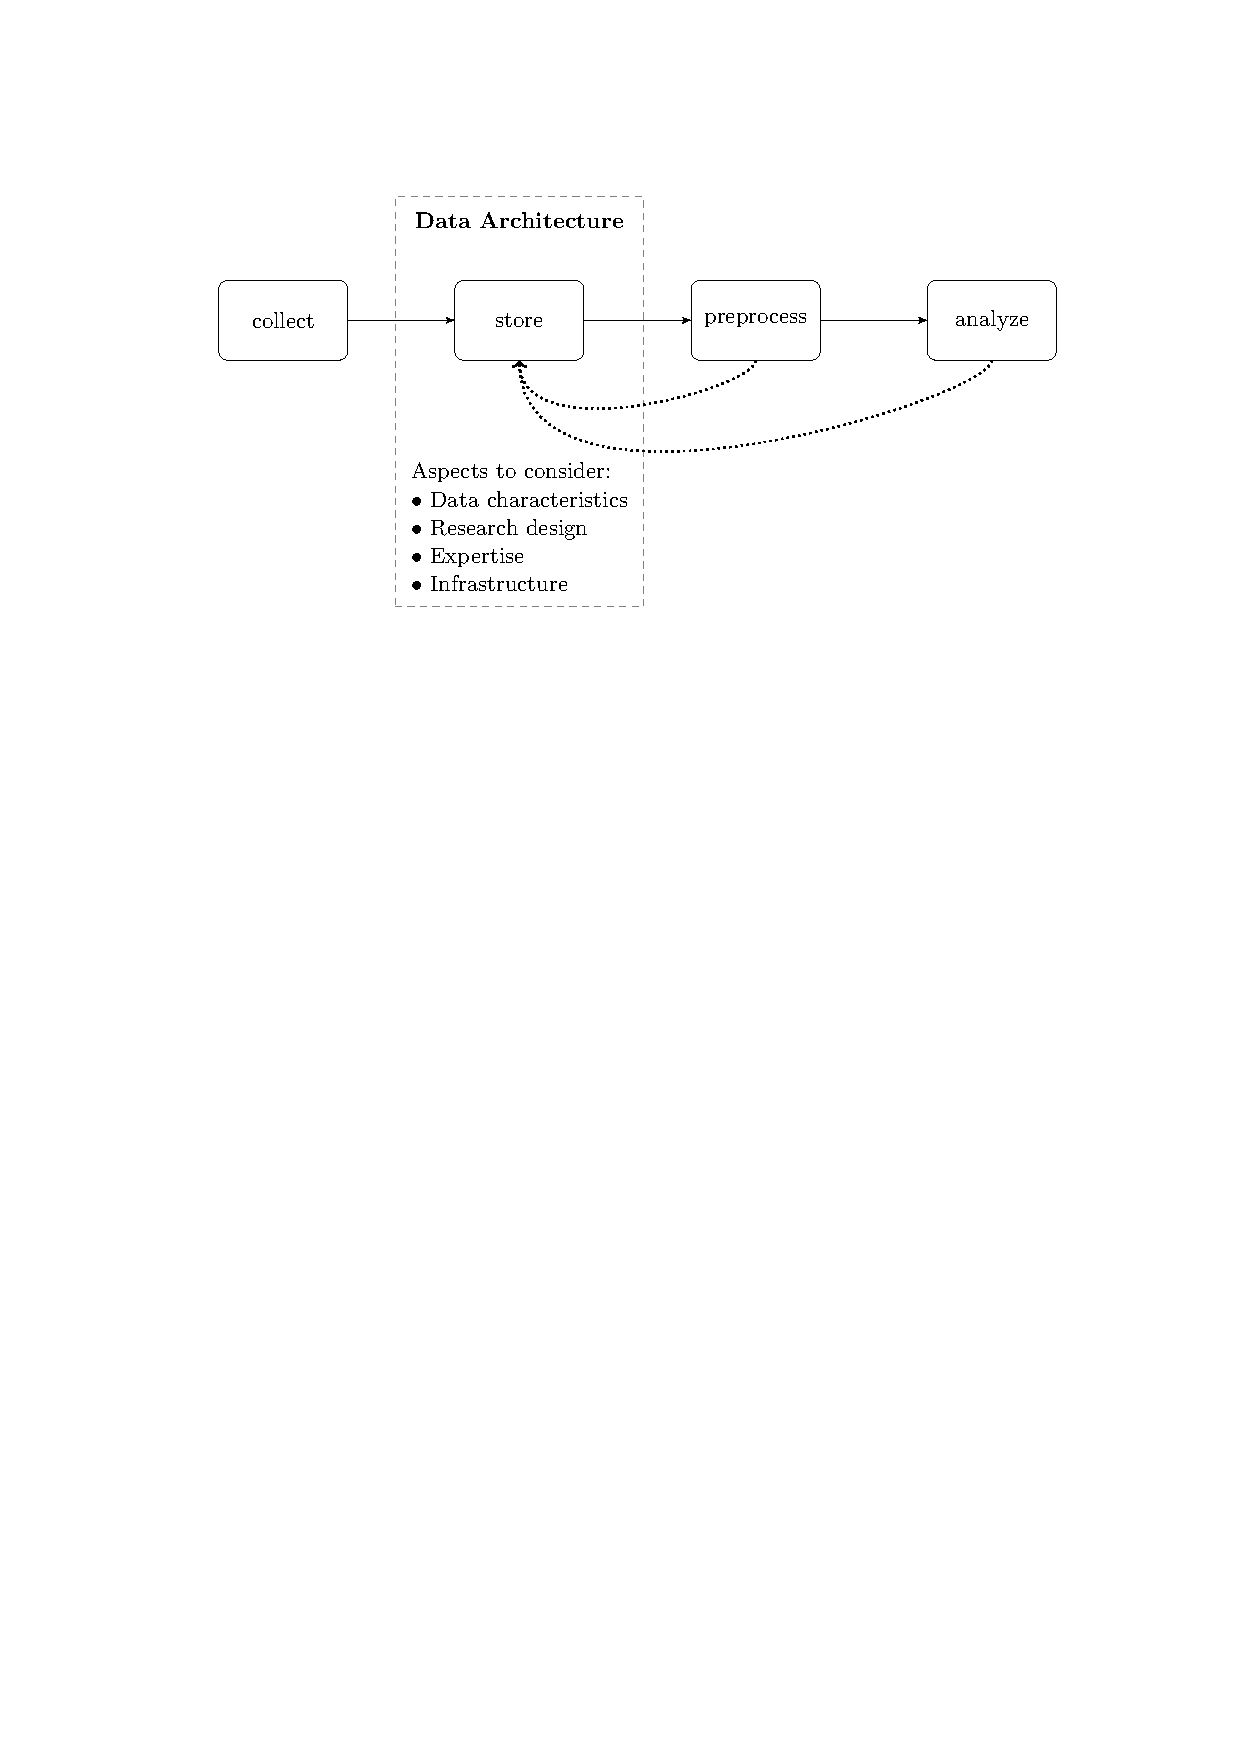
\includegraphics[width=\paperwidth,height=\paperheight,keepaspectratio]{../pictures/guenteretal_fig1}}
\end{frame}

\begin{frame}{From retrieved data to enriched data}
\makebox[\linewidth]{
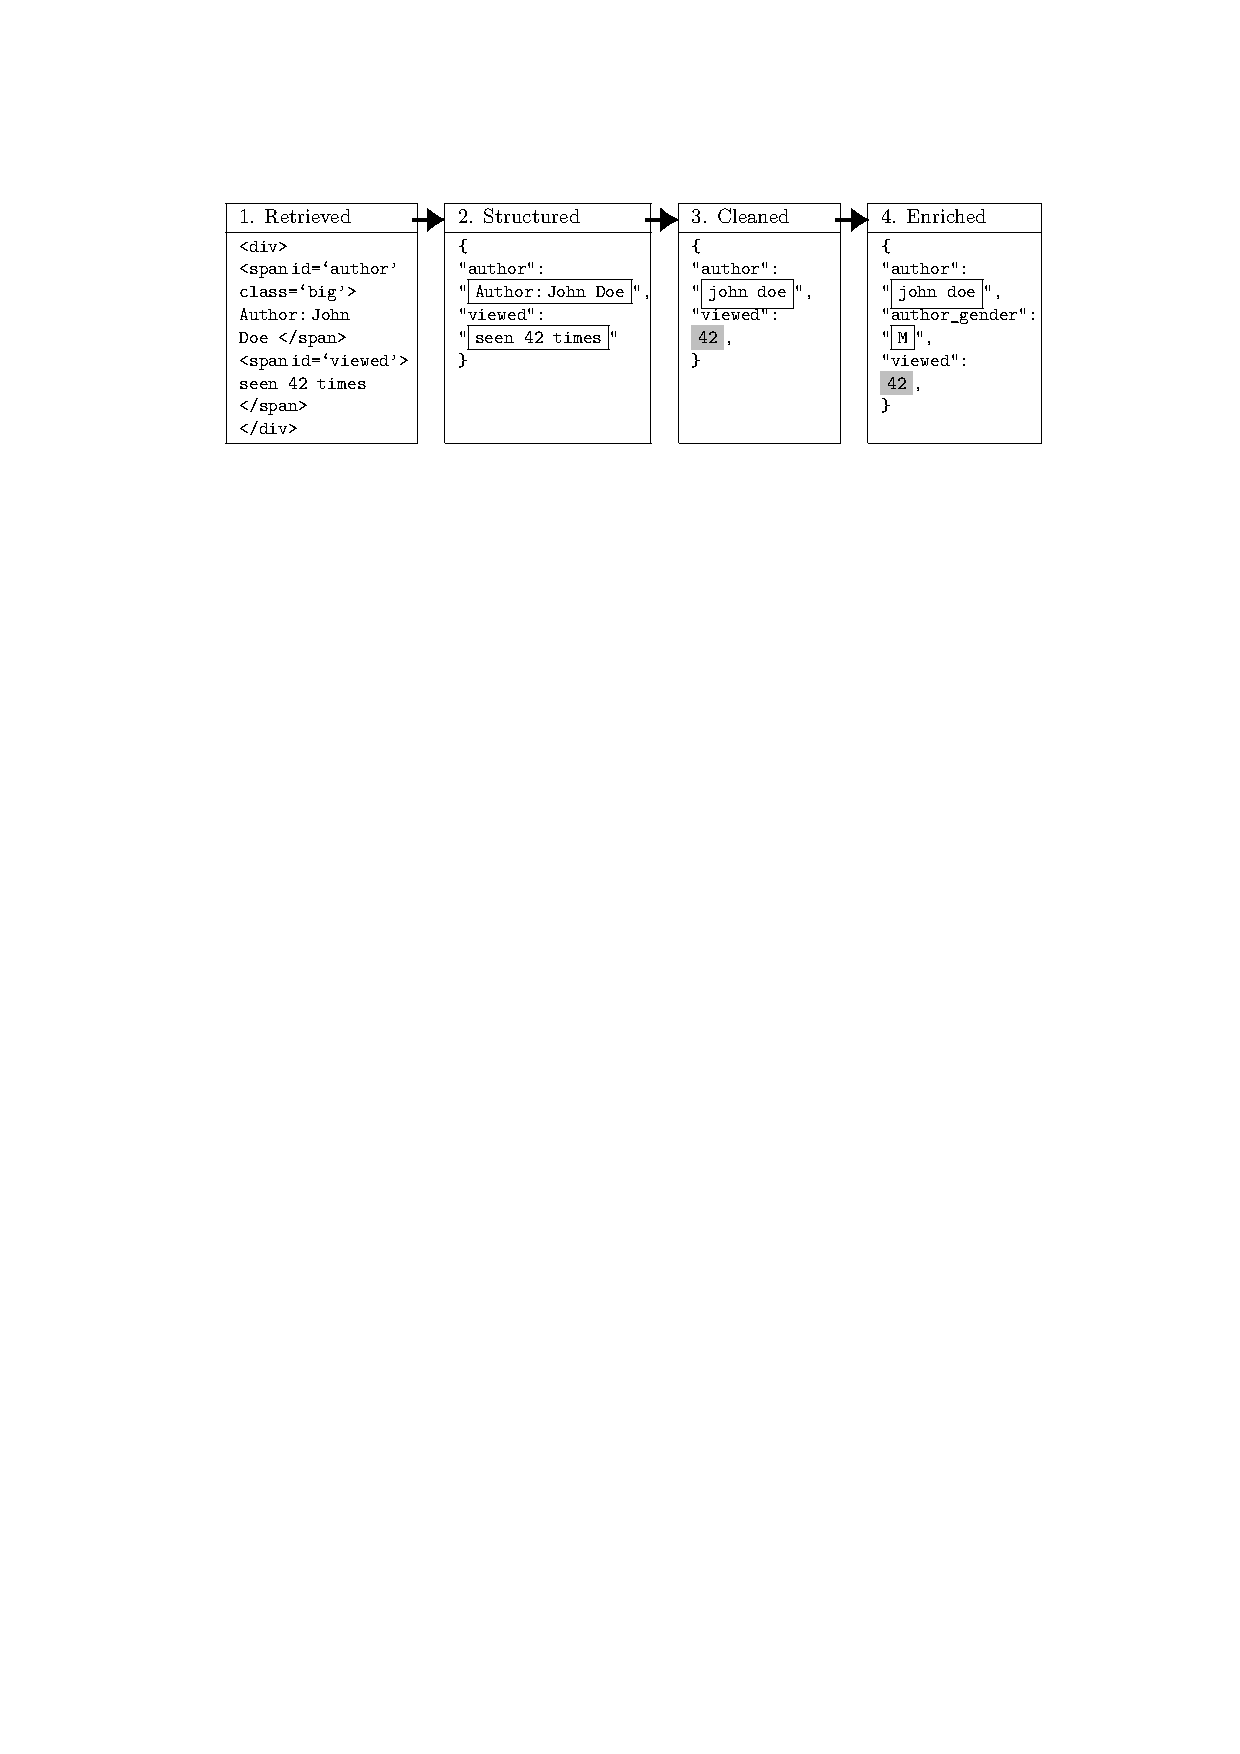
\includegraphics[width=\paperwidth,height=\paperheight,keepaspectratio]{../pictures/guentheretal_fig3}}
\end{frame}


\section{Looking forward}
\subsection{And now you... }
\begin{frame}[plain]{}
Looking forward\\
\textbf{Try to fill in the blanks for your personal CSS project}
\end{frame}


\begin{frame}[plain]
	\begin{tikzpicture}[node distance = 3cm, auto]
	\node [cloud] (retrieve) {retrieve};
	\node [cloud, right of=retrieve] (process) {process and/or enrich};
	\node [cloud, right of=process] (analyze) {analyze\\ explain\\ predict};
	\node [cloud, right of=analyze] (visualize) {communi-cate};
	
	
	\path [pijltje] (retrieve)--(process);
	\path [pijltje] (process)--(analyze);
	\path [pijltje] (analyze)--(visualize);
	
	
	\node [block, below of = retrieve] (retrievetech) {?};
	\node [block, below of= process] (processtech) {?};
	\node [block, below of=analyze] (analyzetech) {?};
	\node [block, below of=visualize] (visualizetech) {?};
	
	
	
	\path [pijltje] (retrievetech)--(processtech);
	\path [pijltje] (processtech)--(analyzetech);
	\path [pijltje] (analyzetech)--(visualizetech);
	
	
	\node [block, below of = retrievetech, fill=green!20] (retrievepython) {?};
	
	\node [block, below of = processtech, fill=green!20] (processpython) {?};
	
	\node [block, below of = analyzetech, fill=green!20] (analyzepython) {?};
	
	\node [block, below of = visualizetech, fill=green!20] (visualizepython) {?};
	
	
	
	
	
	\path [line, dashed] (retrieve)--(retrievetech);
	\path [line, dashed] (process)--(processtech);
	\path [line, dashed] (analyze)--(analyzetech);
	\path [line, dashed] (visualize)--(visualizetech);
	
	
	
	\path [line, dashed] (retrievetech)--(retrievepython);
	\path [line, dashed] (processtech)--(processpython);
	\path [line, dashed] (analyzetech)--(analyzepython);
	\path [line, dashed] (visualizetech)--(visualizepython);
	\end{tikzpicture}
\end{frame}



\begin{frame}[plain]
Long story short:

\textbf{Don't forget to plan the bigger picture}

We will focus on machine learning this week. But for each technique we cover, think about how it fits in \emph{your} workflow.

\pause

\ldots and now lets get started!

\end{frame}

\section[The ACA toolkit]{The Automated Content Analysis toolkit}
\begin{frame}{}
Types of Automated Content Analysis
\end{frame}

\subsection*{Top-down vs. bottom-up}

%{\setbeamercolor{background canvas}{bg=black}
\begin{frame}[plain]
\makebox[\linewidth]{
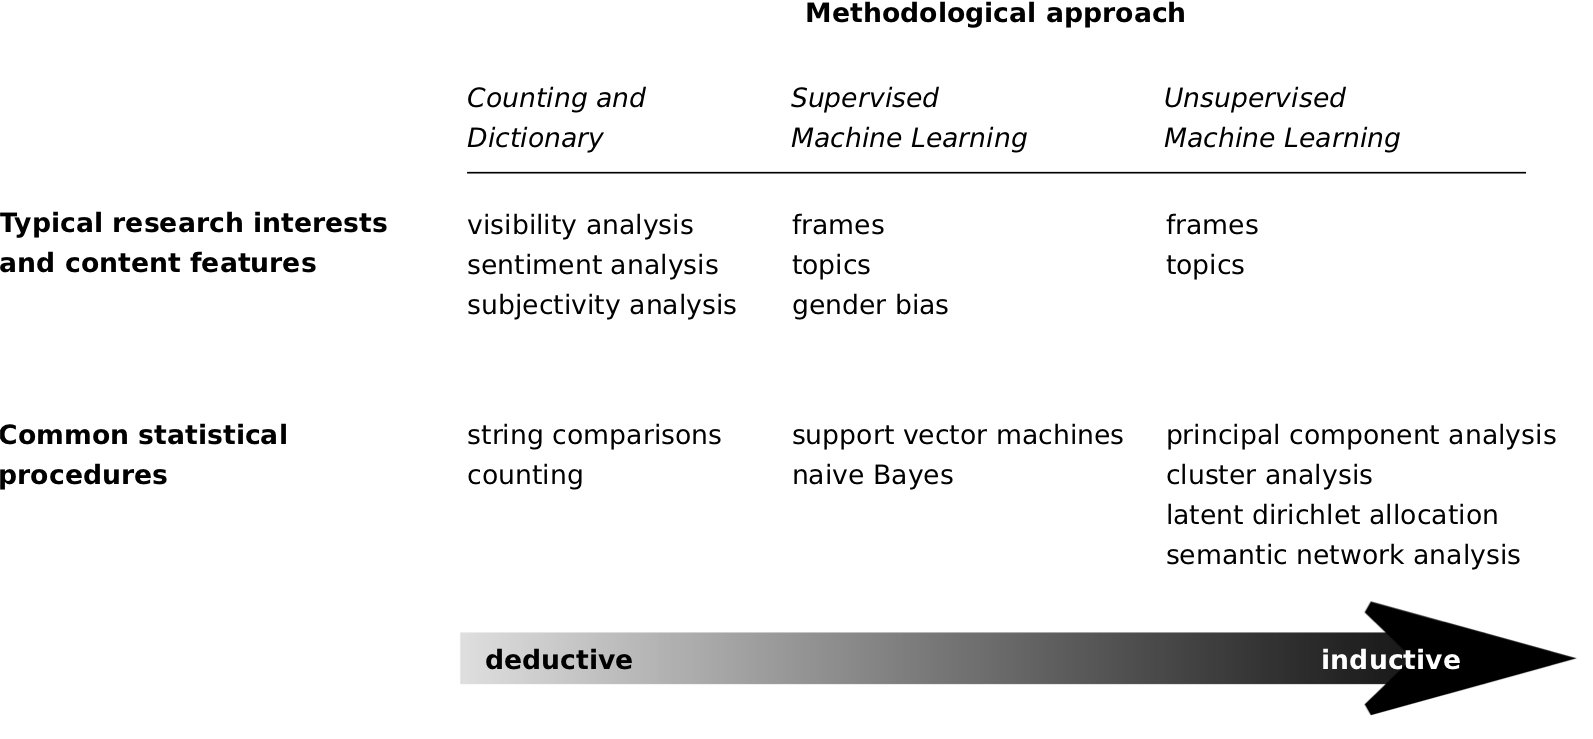
\includegraphics[width=\paperwidth,height=\paperheight,keepaspectratio]{../pictures//boumanstrilling2016_.png}}
\end{frame}
%}

\begin{frame}{Some terminology }
\begin{columns}[t]
\column{.5\textwidth}

\begin{block}<1-4>{Supervised machine learning}
You have a dataset with both predictor and outcome (independent and dependent variables; features and labels) --- a \emph{labeled} dataset.
\onslide<2>{
	\footnotesize{Think of regression: You measured \texttt{x1}, \texttt{x2}, \texttt{x3} and you want to predict \texttt{y}, which you also measured}}
\end{block}

\column{.5\textwidth}

\begin{block}<3->{Unsupervised machine learning}
You have no labels. \onslide<4>{(\footnotesize{You did not measure \texttt{y})}}\\
\onslide<5>{\textbf{Again, you already know some techniques to find out how \texttt{x1}, \texttt{x2},\ldots \texttt{x\_i} co-occur from other courses:} \begin{itemize}
		\item Principal Component Analysis (PCA)
		\item Cluster analysis
		\item \ldots
	\end{itemize}
}
\end{block}

\end{columns}

\end{frame}


\section{Final}

\begin{frame}{This afternoon}
\begin{block}{Getting started}
	Getting started with the IMBD dataset
\end{block}
\end{frame}



\section{Backupslides basics}

\begin{frame}[plain]
\centering
\huge
Backup slides in case we need to do more fundamentals
\end{frame}


\section{Datatypes}


\begin{frame}{Python lingo}
	\begin{block}{Basic datatypes (variables)}
		\begin{description}
			\item[{\color{red}int}] \texttt{37}
			\item[{\color{red}float}] \texttt{1.75}
			\item[{\color{red}bool}] \texttt{True}, \texttt{False}
			\item[{\color{red}string}] \texttt{"Alice"}
			\onslide<2->{\scriptsize \item[({\color{red}variable name}] \texttt{firstname})}
		\end{description}
	\end{block}
	\onslide<2->{\textbf{"firstname" and firstname is not the same.\\}}
	\onslide<3->{\textbf{"5" and 5 is not the same.}\\ But you can transform it: {\tt{int("5")}} will return 5.}\\
	\onslide<3->{\textbf{You cannot calculate \texttt{3 * "5"}} {\tiny{(In fact, you can. It's \tt{"555"})}}.\\
		But you can calculate {\tt{3 * int("5")}}}
\end{frame}



\begin{frame}{Python lingo}
	\begin{block}{More advanced datatypes}
		\begin{description}
			\item[{\color{red}list}]<2-> \texttt{firstnames = ['Alice','Bob','Cecile'] \\
				 lastnames = ['Garcia','Lee','Miller']}
			\item[{\color{red}list}]<3->\texttt{ages = [18,22,45]}
			\item[{\color{red}dict}]<4-> \texttt{agedict = \{'Alice': 18, 'Bob': 22, 'Cecile': 45\} }
		\end{description}
		\onslide<5->{
		Note that the elements of a list, the keys of a dict, and the values of a dict can have any* datatype! (You can even mix them, but it's better to be consistent!)
		
		\tiny{*Well, keys cannot be mutable $\rightarrow$ see book}}
	\end{block}
\end{frame}


\begin{frame}{Python lingo}
	\begin{block}{Retrieving specific items}
		\begin{description}
			\item[{\color{red}list}]<1-> \texttt{firstnames[0]} gives you the first entry\\ 
				\texttt{firstnames[-2]} gives you the one-but-last entry\\
				\texttt{firstnames[:2]} gives you entries 0 and 1\\
				\texttt{firstnames[1:3]} gives you entries 1 and 2\\
				\texttt{firstnames[1:]} gives you entries 1 until the end\\
			\item[{\color{red}dict}]<2-> \texttt{agedict["Alice"]} gives you 18 
		\end{description}
	
	\end{block}
\end{frame}


\question{Think of at least two different ways of storing data about some fictious persons (first name, last name, age, phone number, \ldots) using lists and/or dictionaries. What are the pros and cons?}


\begin{frame}{Python lingo}
	\begin{block}{Less frequent, but still useful datatypes}
		\begin{description}
			\item[{\color{red}set}]A collection in which each item is unique: \texttt{\{1,2,3\}}
			\item[{\color{red}tuple}]Like a list, but \emph{immutable}: \texttt{(1,2,2,2,3)}
			\item[{\color{red}defaultdict}]A dict that does not raise an error but returns the ``empty'' value of its datatype (0 for int, "" for str) if you try access a non-existing key (great for storing results and counting things!)
			\item[{\color{red}np.array}]A list-like datatype provided by the \texttt{numpy} package optimized for efficient mathematical operations.
			\item[$\ldots$]\ldots
		\end{description}
	\end{block}
\small{You will come across more later}
\end{frame}



\section{Functions and methods}
\begin{frame}{Python lingo}
	\begin{block}{Functions}
		\begin{description}
			\item[{\color{red}functions}]<2-> Take an input and return something else \\ {\tt{int(32.43})} returns the integer 32. \texttt{len("Hello")} returns the integer 5.\\ 
			\item[{\color{red}methods}]<3-> are similar to functions, but directly associated with an object. {\tt{"SCREAM".lower()}} returns the string "scream"
		\end{description}
	\end{block}
	\onslide<4->{Both functions and methods end with \texttt{()}. Between the \texttt{()}, \emph{arguments} can (sometimes have to) be supplied.}
\end{frame}



\begin{frame}[fragile]{Some functions}
\begin{lstlisting}
len(x)        # returns the length of x
y = len(x)    # assign the value returned by len(x) to y
print(len(x)) # print the value returned by len(x)
print(y)      # print y
int(x)        # convert x to an integer
str(x)        # convert x to a string
sum(x)        # get the sum of x
\end{lstlisting}
\end{frame}

\question{How could you print the mean (average) of a list of integers using the functions on the previous slide?}



\begin{frame}[fragile]{Some methods}
Some string methods
\begin{lstlisting}
mystring = "Hi! How are you?"
mystring.lower()   # return lowercased string (doesn't change original!)
mylowercasedstring =  mystring.lower()  # save to a new variable
mystring =  mystring.lower()  # or override the old one
mystring.upper()   # uppercase
mystring.split()   # Splits on spaces and returns a list ['Hi!', 'How', 'are', 'you?']
\end{lstlisting}

We'll look into some list methods later.

\textbf{$\Rightarrow$ You can use TAB-completion in Jupyter to see all methods (and properties) of an object!}
\end{frame}


\begin{frame}[fragile]{Writing own functions}
You can write an own function:
\begin{lstlisting}
def addone(x):
    y = x + 1
    return y
\end{lstlisting}

Functions take some input (``argument'') (in this example, we called it \texttt{x}) and \emph{return} some result.

Thus, running
\begin{lstlisting}	
addone(5)
\end{lstlisting}
returns \tt{6}.
\end{frame}

\begin{frame}[fragile]{Writing own functions}

\begin{alertblock}{Attention, R users! (maybe obvious for others?)}
	You \emph{cannot}* apply the function that we just created on a whole list -- after all, it takes an int, not a list as input.
\end{alertblock}

(wait a sec foruntil we cover for loops later today, but this is how you'd do it (by calling the function for each element in the list separately):):

\begin{lstlisting}
mynumbers = [5, 3, 2, 4]
results = [addone(e) for e in mynumbers]
\end{lstlisting}

\vspace{1cm}
\tiny{* Technically speaking, you could do this by wrapping the \texttt{map} function around your own function, but that's not considered ``pythonic''. Don't do it ;-) \\}
\end{frame}




\section[Modifying lists \& dicts]{Modifying lists and dictionaries}
\begin{frame}[fragile]{Modifying lists}
	Let's use one of our first \textcolor{red}{method}s! Each \emph{list} has a method \texttt{.append()}:
\begin{block}{Appending to a list}
\begin{lstlisting}
mijnlijst = ["element 1", "element 2"]
anotherone = "element 3"   # note that this is a string, not a list!
mijnlijst.append(anotherone)
print(mijnlijst)
\end{lstlisting}
gives you:
\begin{lstlisting}
["element 1", "element 2", "element 3"]
\end{lstlisting}
\end{block}
\end{frame}



\begin{frame}[fragile]{Modifying lists}
\begin{block}{Merging two lists (= extending)}
\begin{lstlisting}
mijnlijst = ["element 1", "element 2"]
anotherone = ["element 3", "element 4"]
mijnlist.extend(anotherone)
print(mijnlijst)
\end{lstlisting}
gives you:
\begin{lstlisting}
["element 1", "element 2", "element 3", "element 4]
\end{lstlisting}
\end{block}
\end{frame}

\question{What would have happened if we had used \texttt{.append()} instead of \texttt{.extend()}?}

\question{Why do you think that the Python developers implemented \texttt{.append()} and \texttt{.extend()} as methods of a list and not as functions?}


\begin{frame}[fragile]{Modifying dicts}
\begin{block}{Adding a key to a dict (or changing the value of an existing key)}
\begin{lstlisting}
mydict = {"whatever": 42, "something": 11}
mydict["somethingelse"] = 76
print(mydict)
\end{lstlisting}
gives you:
\begin{lstlisting}
{'whatever': 42, 'somethingelse': 76, 'something': 11}
\end{lstlisting}
If a key already exists, its value is simply replaced.
\end{block}
\end{frame}




\section{for, if/elif/else, try/except}

\begin{frame}[fragile]{How can we structure our program?}
If we want to \emph{repeat} a block of code, exectute a block of code only \emph{under specific conditions}, or more generally want to structure our code, we use \emph{indention}.

	\begin{block}{Indention: The Python way of structuring your program}
		\begin{itemize}
			\item Your program is structured by TABs or SPACEs.
			\item Jupyter (or your IDE) handles (guesses) this for you, but make sure to not interfere and not to mix TABs or SPACEs!
			\item Default: four spaces per level of indention.
		\end{itemize}
	\end{block}
\end{frame}



\begin{frame}[fragile]{Indention}
\begin{block}{Structure}
	A first example of an indented block -- in this case, we want to \emph{repeat} this block:
\end{block}
\begin{lstlisting}
agedict = {'Zeus': None, 'Denis': 96, 'Alice': 18, 'Rebecca': 20 , 'Bob': 22, 'Cecile': 45}

myfriends = ['Alice','Bob','Cecile']

print ("The names and ages of my friends:")
for buddy in myfriends:
	print (f"My friend {buddy} is {agedict[buddy]} years old")
\end{lstlisting}

Output:
\begin{lstlisting}
My friend Alice is 18 years old
My friend Bob is 22 years old
My friend Cecile is 45 years old
\end{lstlisting}
\end{frame}

\begin{frame}[fragile]{What happened here?}

\begin{lstlisting}
for buddy in myfriends:
    print (f"My friend {buddy} is {agedict[buddy]} years old")
\end{lstlisting}

\small
	\begin{block}{The for loop}
\begin{enumerate}
	\item Take the first element from \texttt{myfriends} and call it \texttt{buddy} (like \texttt{buddy = myfriends[0]}) (line 1)
	\item Execute the indented block (line 2, but could be more lines)
	\item Go back to line 1, take next element  (like \texttt{buddy = myfriends[1]}) 
	\item Execture the indented block \ldots
	\item \ldots repeat until no elements are left \ldots
\end{enumerate}
	\end{block}
	
	\begin{block}{The f-string (\emph{formatted} string)}
If you prepend a string with an \texttt{f}, you can use curly brackets texttt{\{\}} to insert the value of a variable
	\end{block}
	
\end{frame}




\begin{frame}[fragile]{What happened here?}
\begin{lstlisting}
for buddy in myfriends:
    print (f"My friend {buddy} is {agedict[buddy]} years old")
\end{lstlisting}
\small
The line \emph{before} an indented block starts with a \emph{statement} indicating what should be done with the block and ends with a \texttt{:}

\footnotesize
\begin{block}{More in general, the \texttt{:} + indention indicates that}<2->
	\begin{itemize}
		\item<3-> the block is to be executed repeatedly (\texttt{for} statement) – e.g., for each element from a list, or until a condition is reached (\texttt{while} statement)
		\item<4-> the block is only to be executed under specific conditions (\texttt{if}, \texttt{elif}, and \texttt{else} statements)
		\item<5-> an alternative block should be executed if an error occurs in the block (\texttt{try} and \texttt{except} statements)
		\item<6-> a file is opened, but should be closed again after the block has been executed (\texttt{with} statement)
	\end{itemize}
\end{block}
\end{frame}



\begin{frame}[fragile]{Can we also loop over dicts?}
Sure! But we need to indicate how exactly:

\begin{lstlisting}
mydict = {"A":100, "B": 60, "C": 30}

for k in mydict:   # or mydict.keys()
    print(k)

for v in mydict.values():
    print(v)

for k,v in mydict.items():
    print(f"{k} has the value {v}")
\end{lstlisting}

\end{frame}




\begin{frame}[fragile]{Can we also loop over dicts?}
The result:

\begin{lstlisting}
A
B
C

100
60
30

A has the value 100
B has the value 60
C has the value 30
\end{lstlisting}

\end{frame}



\begin{frame}[fragile]{if statements}
	\begin{block}{Structure}
		Only execute block if condition is met
	\end{block}
	\begin{lstlisting}
x = 5
if x <10:
   print(f"{x} is smaller than 10")
elif x > 20:
   print(f"{x} is greater than 20")
else:
   print("No previous condition is met, therefore 10<={x}<=20")
\end{lstlisting}

\end{frame}


\question{Can you see how such an if statement could be particularly useful when nested in a for loop?}



\begin{frame}[fragile]{try/except}
\begin{block}{Structure}
If executed block fails, run another block instead
\end{block}
\begin{lstlisting}
x = "5"
try: 
   myint = int(x)
except:
   myint = 0
\end{lstlisting}

\pause 
\small{Again, more useful when executed repeatedly (in a loop or function):}
\begin{lstlisting}
mylist = ["5", 3, "whatever", 2.2]
myresults = []
for x in mylist:
    try: 
        myresults.append(int(x))
    except:
        myresults.append(None)
print(myresults)
\end{lstlisting}
\end{frame}





\section{Bonus: Python goodies}

\begin{frame}[fragile]{List comprehensions}
\begin{block}{Structure}
A for loop that \texttt{.append()}s to an empty list can be replaced by a one-liner:
\end{block}
\begin{lstlisting}
mynumbers = [2,1,6,5]
mysquarednumbers = []
for x in mynumbers:
    mysquarednumbers.append(x**2))
\end{lstlisting}
is equivalent to:
\begin{lstlisting}
mynumbers = [2,1,6,5]
mysquarednumbers = [x**2 for x in mynumbers]
\end{lstlisting}

\pause 
Optionally, we can have a condition:
\begin{lstlisting}
mynumbers = [2,1,6,5]
mysquarednumbers = [x**2 for x in mynumbers if x>3]
\end{lstlisting}

\end{frame}




\begin{frame}[fragile]{List comprehensions}
	\begin{alertblock}{A very pythonic construct}
		\begin{itemize}
			\item Every for loop can also be written as a for loop that appends to a new list to collect the results. 
			\item For very complex operations (e.g., nested for loops), it can be easier to write out the full loops. 
			\item But mostly, list comprehensions are really great! (and much more concise!)
		\end{itemize}
	\end{alertblock}
\textbf{$\Rightarrow$ You really should learn this!}
	\end{frame}



\begin{frame}[fragile]{Generators}
\begin{block}{Structure}
	A lazy for loop (or function) that only generates its next element when it is needed:
\end{block}
\footnotesize
You can create a generator just like a list comprehension (but with \texttt{()} instead of \texttt{[]}):
\begin{lstlisting}
mynumbers = [2,1,6,5]
squaregen = (x**2 for x in mynumbers)   # these are NOT calculated yet
for e in squaregen:
    print(e)             # only here, we are calculating the NEXT item
\end{lstlisting}
\pause
Or like a function (but with \texttt{yield} instead of \texttt{return}):
\begin{lstlisting}
def squaregen(listofnumbers):
    for x in listofnumbers:
        yield(x**2)
mygen = squaregen(mynumbers)
for e in mygen:
    print(e)
\end{lstlisting}

\end{frame}


\begin{frame}[fragile]{Generators}
	\begin{alertblock}{A very memory and time efficient construct}
		\begin{itemize}
			\item Every function that \emph{returns} a list can also be written as a generator that \emph{yields} the elements of the list
			\item Especially useful if
			\begin{itemize}
				\item it takes a long time to calculate the list
				\item the list is very large and uses a lot of memory (hi big data!)
				\item the elements in the list are fetched from a slow source (a file, a network connection)
				\item you don't know whether you actually will need all elements
			\end{itemize}
		\end{itemize}

		\end{alertblock}
		\textbf{$\Rightarrow$ You probably don't need this right now, but (a) it will come in very handy once you deal with web scraping or very large collections, and (b) you may come across generators in some examples}
		\end{frame}



\begin{frame}[standout]
	Make sure you understood all of today's concepts.
	
	Also read Chapter 4 and ask questions if needed.
	If you want do some exercises with basic python, please see here:
	 \large{\url{https://github.com/annekroon/gesis-machine-learning/blob/main/day1/exercises-basicpython/exercises.md}}
\end{frame}




\end{document}

